





%----------------------------------------------------------------------------------------

\newpage

%%%%%%%%%%%%%%%%%%%%%%%
\section{Exploration of the SimpopNet model}{Exploration du modèle SimpopNet}

\label{app:sec:macrocoevolexplo}


\bpar{
We give here supplementary figures that allow rendering the sensitivity of results to parameters not presented in main text.
}{
Nous donnons ici des figures supplémentaires permettant de se rendre compte de la sensibilité des résultats aux paramètres non présentés en texte principal.
}


\bpar{
The Fig~\ref{fig:app:macrocoevolexplo:closeness} allows visualizing the sensitivity of the entropy of centralities $\varepsilon \left[\mu_i\right]$ as a function of $d_G$, $\theta_N$ and $\gamma_G$. The shape of temporal curves is mainly sensitive to $\gamma_G$.
}{
La Fig.~\ref{fig:app:macrocoevolexplo:closeness} permet de visualiser la sensibilité de l'entropie des centralités $\varepsilon \left[\mu_i\right]$ en fonction de $d_G$, $\theta_N$ et $\gamma_G$. La forme des courbes temporelles est principalement sensible à $\gamma_G$.
}


%%%%%%%%%%%%%%%%%
\begin{figure}
    %\includegraphics[width=0.48\linewidth]{Figures/MacroCoEvolExplo/closenessEntropies_networkGamma2_5_networkSpeed110.pdf}
    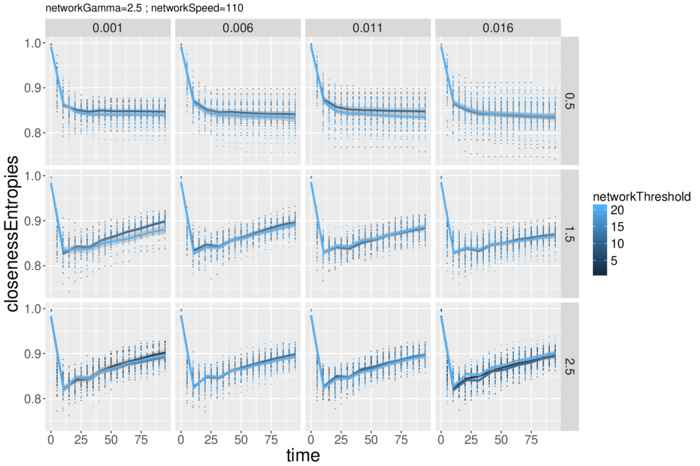
\includegraphics[width=\linewidth]{Figures/Final/A-macrocoevolexplo-closeness.jpg}
\appcaption{\textbf{Entropy of closeness centralities.} We give $\varepsilon \left[\mu_i\right]$ as a function of time $t$, for $\theta_N$ variable (color), $d_G$ variable (columns) and $\gamma_G$ variable.\label{fig:app:macrocoevolexplo:closeness}}{\textbf{Entropie des centralités de proximité.} Nous donnons $\varepsilon \left[\mu_i\right]$ en fonction du temps $t$, pour $\theta_N$ variable (couleur), $d_G$ variable (colonnes) et $\gamma_G$ variable.\label{fig:app:macrocoevolexplo:closeness}}
\end{figure}
%%%%%%%%%%%%%%%%%


\bpar{
The Fig.~\ref{fig:app:macrocoevolexplo:rankcorrpop} gives the variations of $\rho_r$ as a function of $d_G$ and $\gamma_G$, for variable values of $\theta_N$ and of $\gamma_N$. We see that the regularity observed as a function of $d_G$ and of $\gamma_G$ appears not to be sensitive to the variations of $\theta_N$ and of $\gamma_N$.
}{
La Fig.~\ref{fig:app:macrocoevolexplo:rankcorrpop} donne les variations de $\rho_r$ en fonction de $d_G$ et $\gamma_G$, pour des valeurs variables de $\theta_N$ et de $\gamma_N$. Nous constatons que la régularité observée en fonction de $d_G$ et de $\gamma_G$ n'est pas visiblement sensible aux variations de $\theta_N$ et de $\gamma_N$.
}


%%%%%%%%%%%%%%%%%
\begin{figure}
    %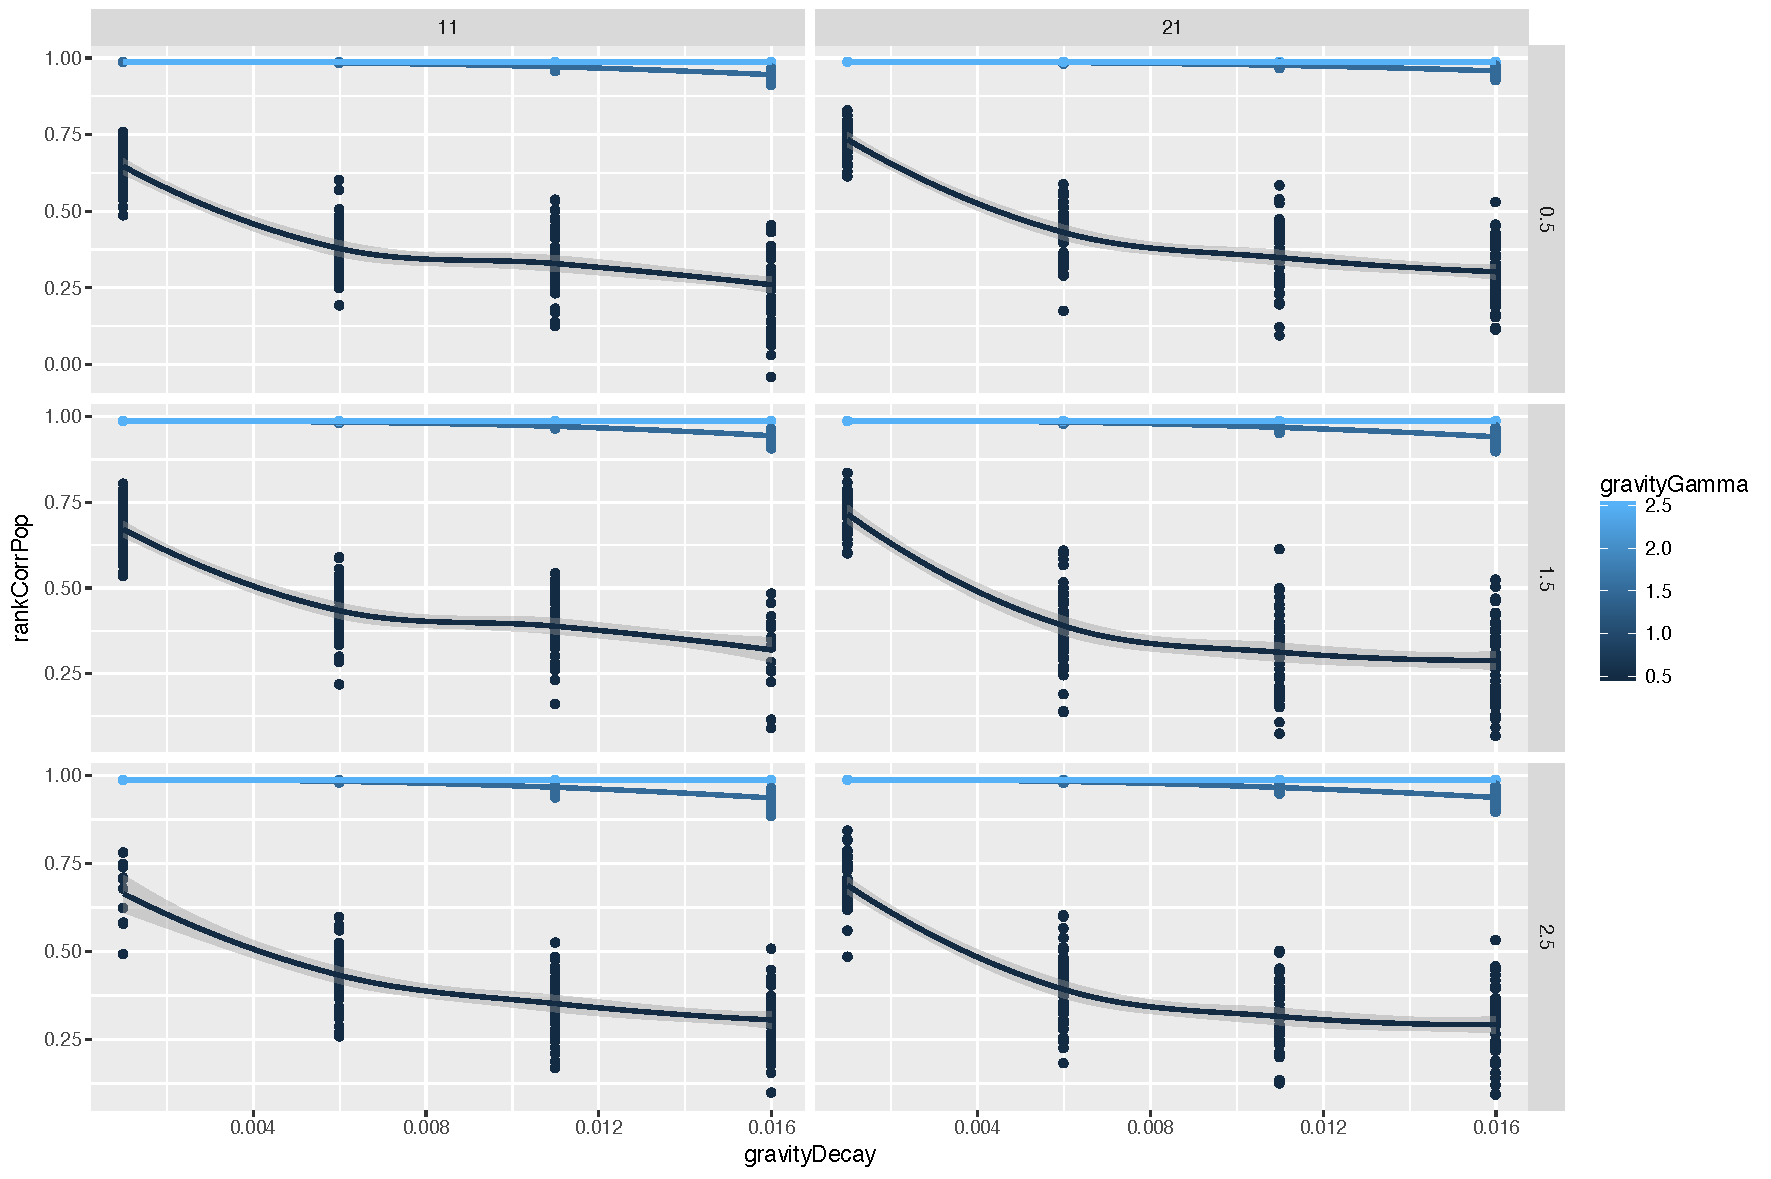
\includegraphics[width=0.48\linewidth]{Figures/MacroCoEvolExplo/rankCorrPop_synthRankSize0_5_networkSpeed10}
    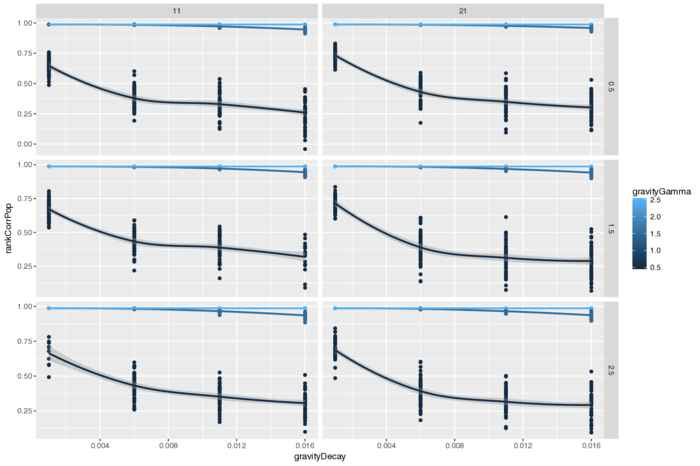
\includegraphics[width=\linewidth]{Figures/Final/A-macrocoevolexplo-rankcorrpop.jpg}
\appcaption{\textbf{Population rank correlations.} We give $\rho_r \left[\mu_i\right]$ as a function of $d_G$, for $\gamma_G$ variable (color), $\theta_N$ variable (columns) and $\gamma_N$ variable (rows).\label{fig:app:macrocoevolexplo:rankcorrpop}}{\textbf{Corrélations de rang pour la population.} Nous donnons $\rho_r \left[\mu_i\right]$ en fonction de $d_G$, pour $\gamma_G$ variable (couleur), $\theta_N$ variable (colonnes) et $\gamma_N$ variable (lignes).\label{fig:app:macrocoevolexplo:rankcorrpop}}
\end{figure}
%%%%%%%%%%%%%%%%%


\bpar{
The Fig.~\ref{fig:app:macrocoevolexplo:distcorrs} gives correlations $\rho_d$ as a function of distance for all couples of variables, for varying $d_G$ and $\gamma_G$. We obtain qualitatively the same behaviors than with $d_G = 0.016$, at the exception of a very low growth for the largest distances, for the correlation between population and accessibility, at $d_G=0.001$ and $\gamma_G = 0.5$, which remains difficult to interpret.
}{
La Fig.~\ref{fig:app:macrocoevolexplo:distcorrs} donne les corrélations $\rho_d$ en fonction de la distance pour l'ensemble des couples de variables, pour $d_G$ et $\gamma_G$ variables. Nous retrouvons qualitativement les mêmes comportements que avec $d_G = 0.016$, à l'exception d'une très légère croissance pour les plus grande distances, pour la corrélation entre la population et l'accessibilité, à $d_G=0.001$ et $\gamma_G = 0.5$, qui reste difficile à interpréter.
}



%%%%%%%%%%%%%%%%%
\begin{figure}
	%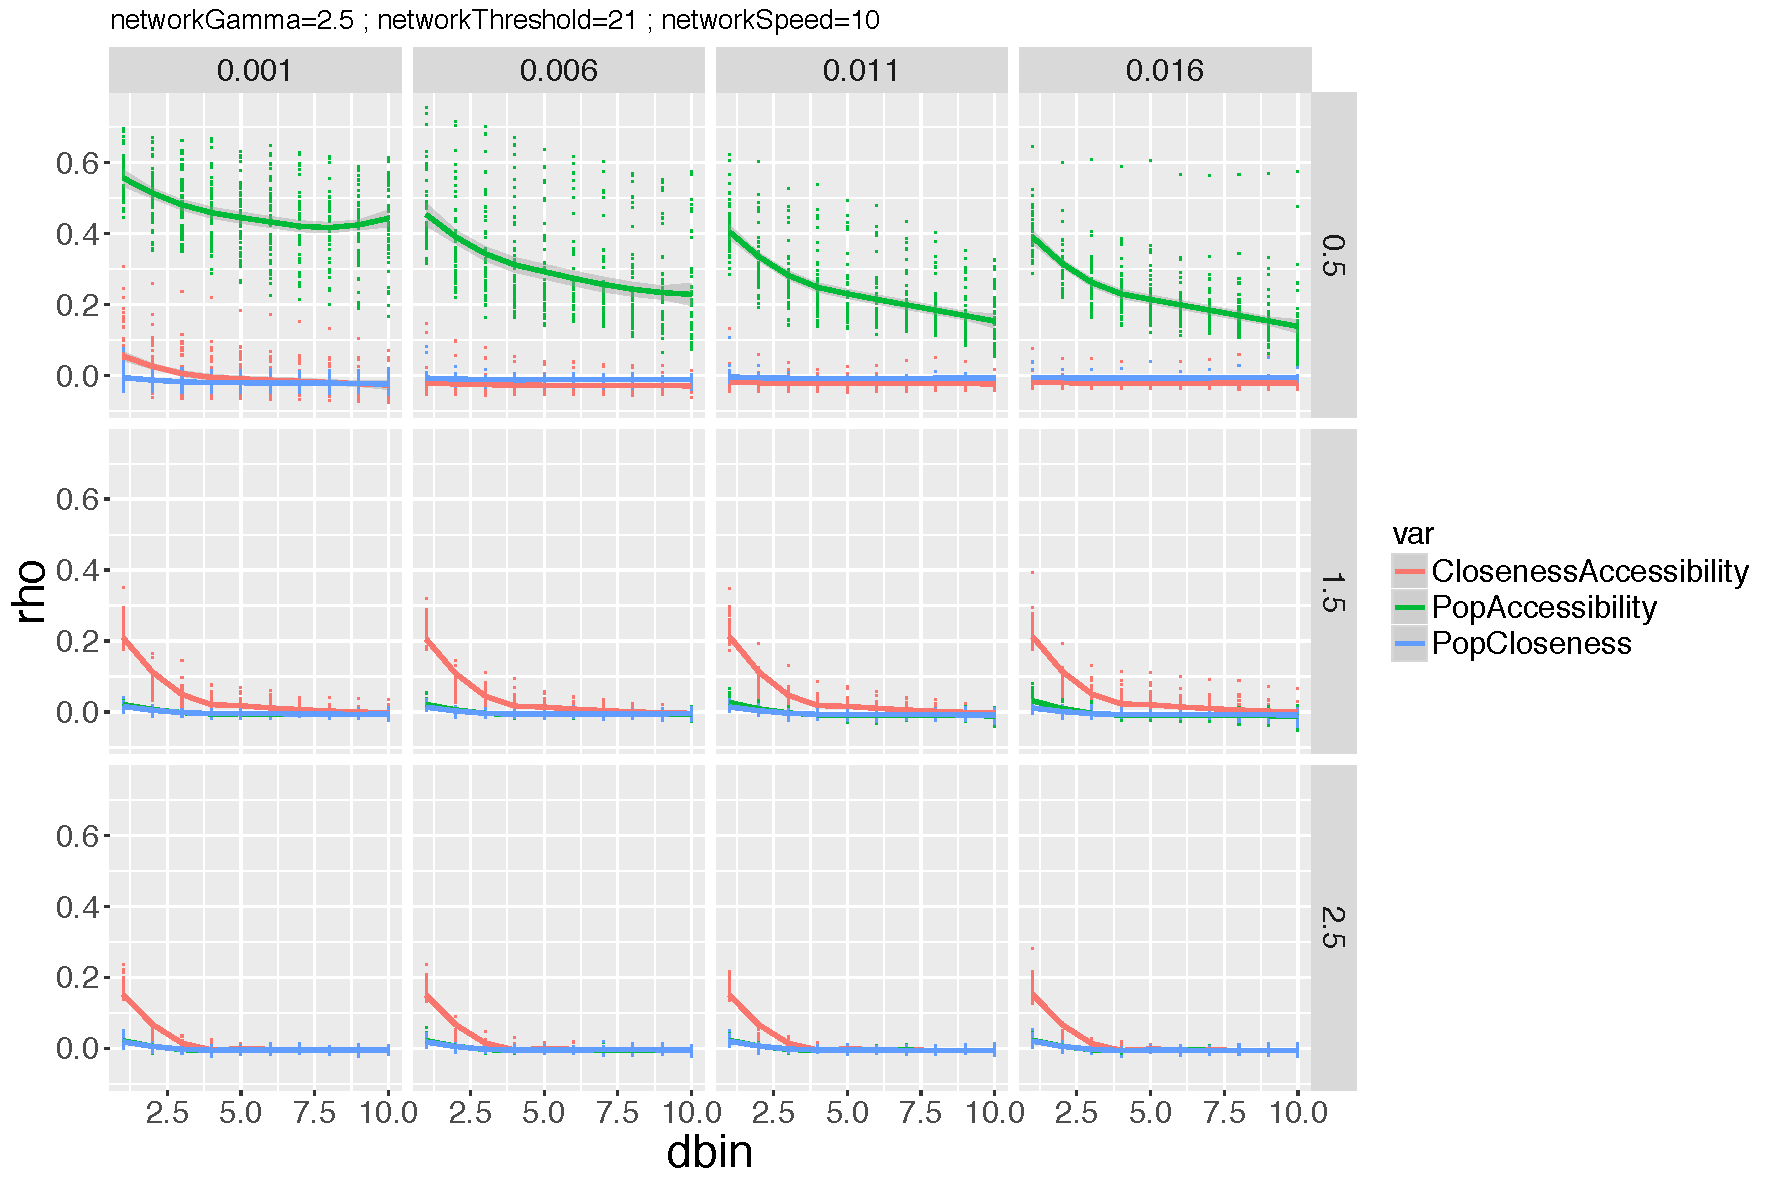
\includegraphics[width=0.48\linewidth]{Figures/MacroCoEvolExplo/distcorrs_networkGamma2_5_networkThreshold21_networkSpeed10}
	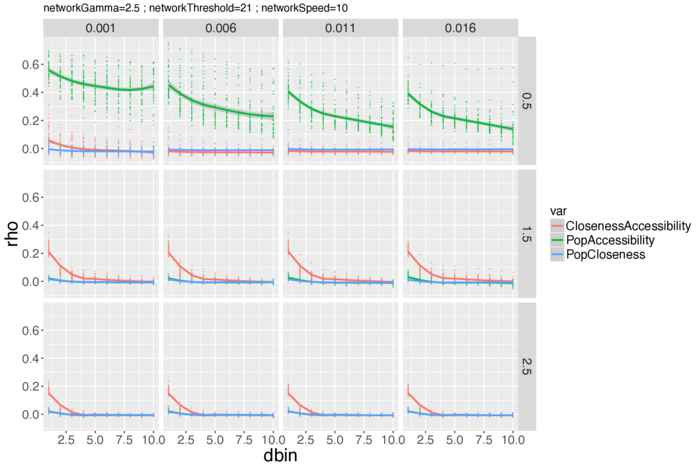
\includegraphics[width=\linewidth]{Figures/Final/A-macrocoevolexplo-distcorrs.jpg}
	\appcaption{\textbf{Correlations as a function of distance.} We give correlations $\rho_d$ as a function of distance decile, for all couples of variables (color), for $d_G$ variable (columns) and $\gamma_G$ variable (rows), at fixed $\gamma_N = 2.5$, $\theta_N=21$ and $v_0 = 10$.\label{fig:app:macrocoevolexplo:distcorrs}}{\textbf{Corrélations en fonction de la distance.} Nous donnons les corrélations $\rho_d$ en fonction du décile de la distance, pour l'ensemble des couples de variables (couleur), pour $d_G$ variable (colonnes) et $\gamma_G$ variable (lignes), à $\gamma_N = 2.5$, $\theta_N=21$ et $v_0 = 10$ fixés.\label{fig:app:macrocoevolexplo:distcorrs}}
\end{figure}
%%%%%%%%%%%%%%%%%


\bpar{
Finally, we give in Fig.~\ref{fig:app:macrocoevolexplo:laggedcorrs} the lagged correlations $\rho_{\tau}$ between all couples of variables, for varying $d_G$ and $\gamma_G$. Similarly, qualitative behaviors are globally stable for other parameters than $\gamma_G$.
}{
Enfin, nous donnons en Fig.~\ref{fig:app:macrocoevolexplo:laggedcorrs} les corrélations retardées $\rho_{\tau}$ entre l'ensemble des couples de variables, pour $d_G$ et $\gamma_G$ variables. De même, les comportements qualitatifs sont globalement stables pour les paramètres autres que $\gamma_G$.
}


%%%%%%%%%%%%%%%%%
\begin{figure}
	%\includegraphics[width=0.48\linewidth]{Figures/MacroCoEvolExplo/laggedcorrs_networkGamma2_5_networkThreshold21_networkSpeed10}
	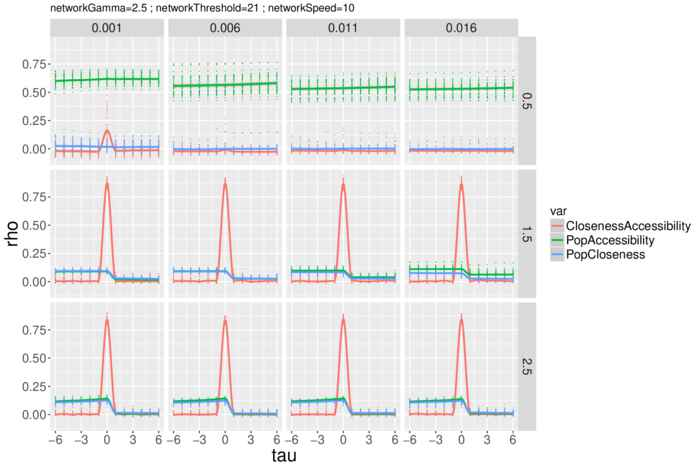
\includegraphics[width=\linewidth]{Figures/Final/A-macrocoevolexplo-laggedcorrs.jpg}
	\appcaption{\textbf{Lagged correlations.} We give the lagged correlations $\rho_{\tau}$ as a function of the delay $\tau$, for all couples of variables (color), for $d_G$ variable (columns) and $\gamma_G$ variable (rows), at fixed $\gamma_N = 2.5$, $\theta_N=21$ and $v_0 = 10$.\label{fig:app:macrocoevolexplo:laggedcorrs}}{\textbf{Corrélations retardées.} Nous donnons les corrélations retardées $\rho_{\tau}$ en fonction du délai $\tau$, pour l'ensemble des couples de variables (couleur), pour $d_G$ variable (colonnes) et $\gamma_G$ variable (lignes), à $\gamma_N = 2.5$, $\theta_N=21$ et $v_0 = 10$ fixés.\label{fig:app:macrocoevolexplo:laggedcorrs}}
\end{figure}
%%%%%%%%%%%%%%%%%




%----------------------------------------------------------------------------------------

\newpage

%%%%%%%%%%%%%%%%%%%%%%%
\section{Macroscopic co-evolution model}{Modèle de co-évolution macroscopique}

\label{app:sec:macrocoevol}



%%%%%%%%%%%%%%%%%%%
\subsection{Synthetic data}{Données synthétiques}


\subsubsection{Exploration}{Exploration}


\bpar{
we give in Fig.~\ref{fig:app:macrocoevol:behavior-time} the sensitivity of temporal indicators for the co-evolution model on synthetic data, in particular $\bar{c_i}(t)$ and $\varepsilon\left[\mu_i\right](t)$, for variations of $d_G$, $\gamma_G$ and $\phi_0$. The behavior of $\bar{c_i}$  is sensitive to $\gamma_G$ et $\phi_0$ but not much to $d_G$. The one of $\varepsilon\left[\mu_i\right]$ does depend only on $\gamma_G$ for its average behavior, and on $d_G$ for its dispersion in low $d_G$ values.
}{
Nous donnons en Fig.~\ref{fig:app:macrocoevol:behavior-time} la sensibilité des indicateurs temporels pour le modèle de co-évolution sur données synthétiques, en particulier $\bar{c_i}(t)$ et $\varepsilon\left[\mu_i\right](t)$, pour des variations de $d_G$, $\gamma_G$ et $\phi_0$. Le comportement de $\bar{c_i}$ est sensible à $\gamma_G$ et $\phi_0$ mais très peu à $d_G$. Celui de $\varepsilon\left[\mu_i\right]$ ne dépend que de $\gamma_G$ pour son comportement moyen, et de $d_G$ pour sa dispersion dans les faibles valeurs de $d_G$.
}


%%%%%%%%%%%%%
\begin{figure}
%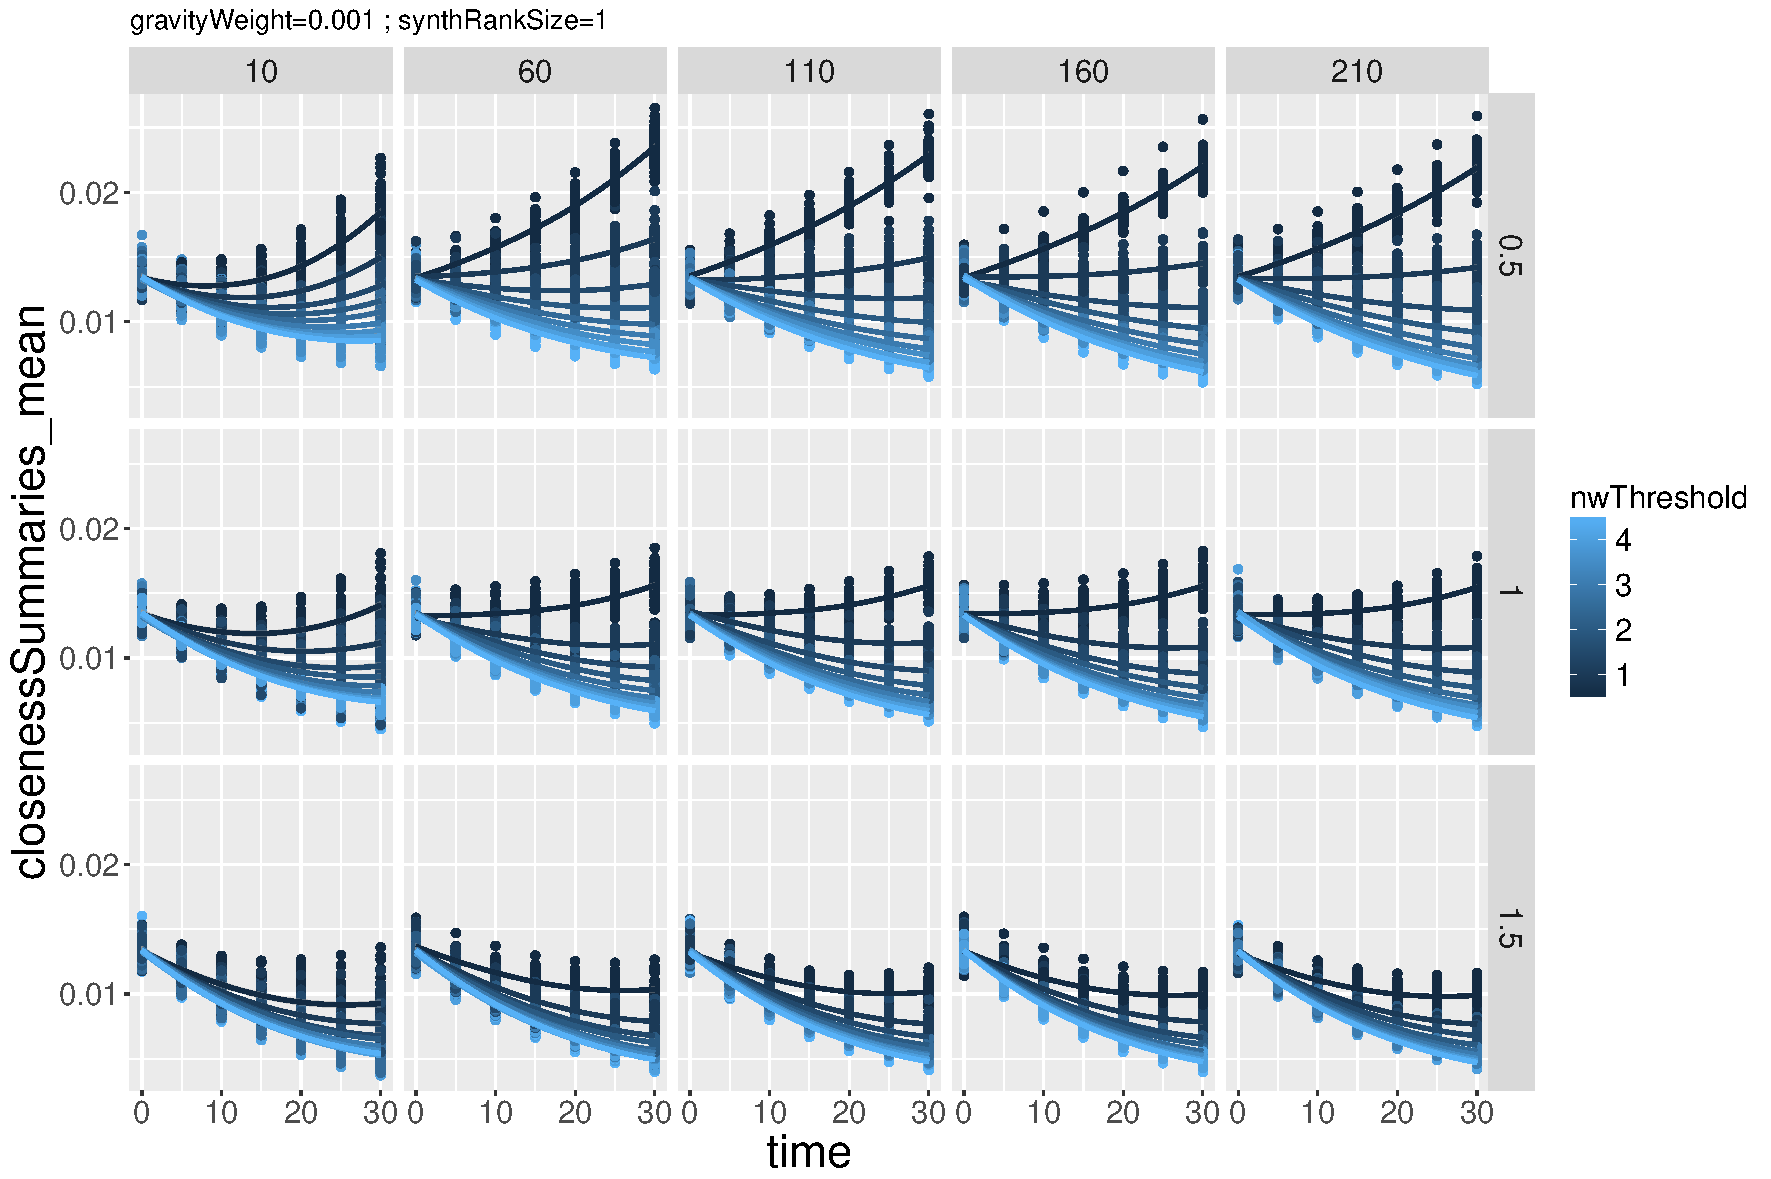
\includegraphics[width=0.48\linewidth]{Figures/MacroCoEvol/closenessSummaries_meansynthRankSize1_gravityWeight0_001.pdf}
%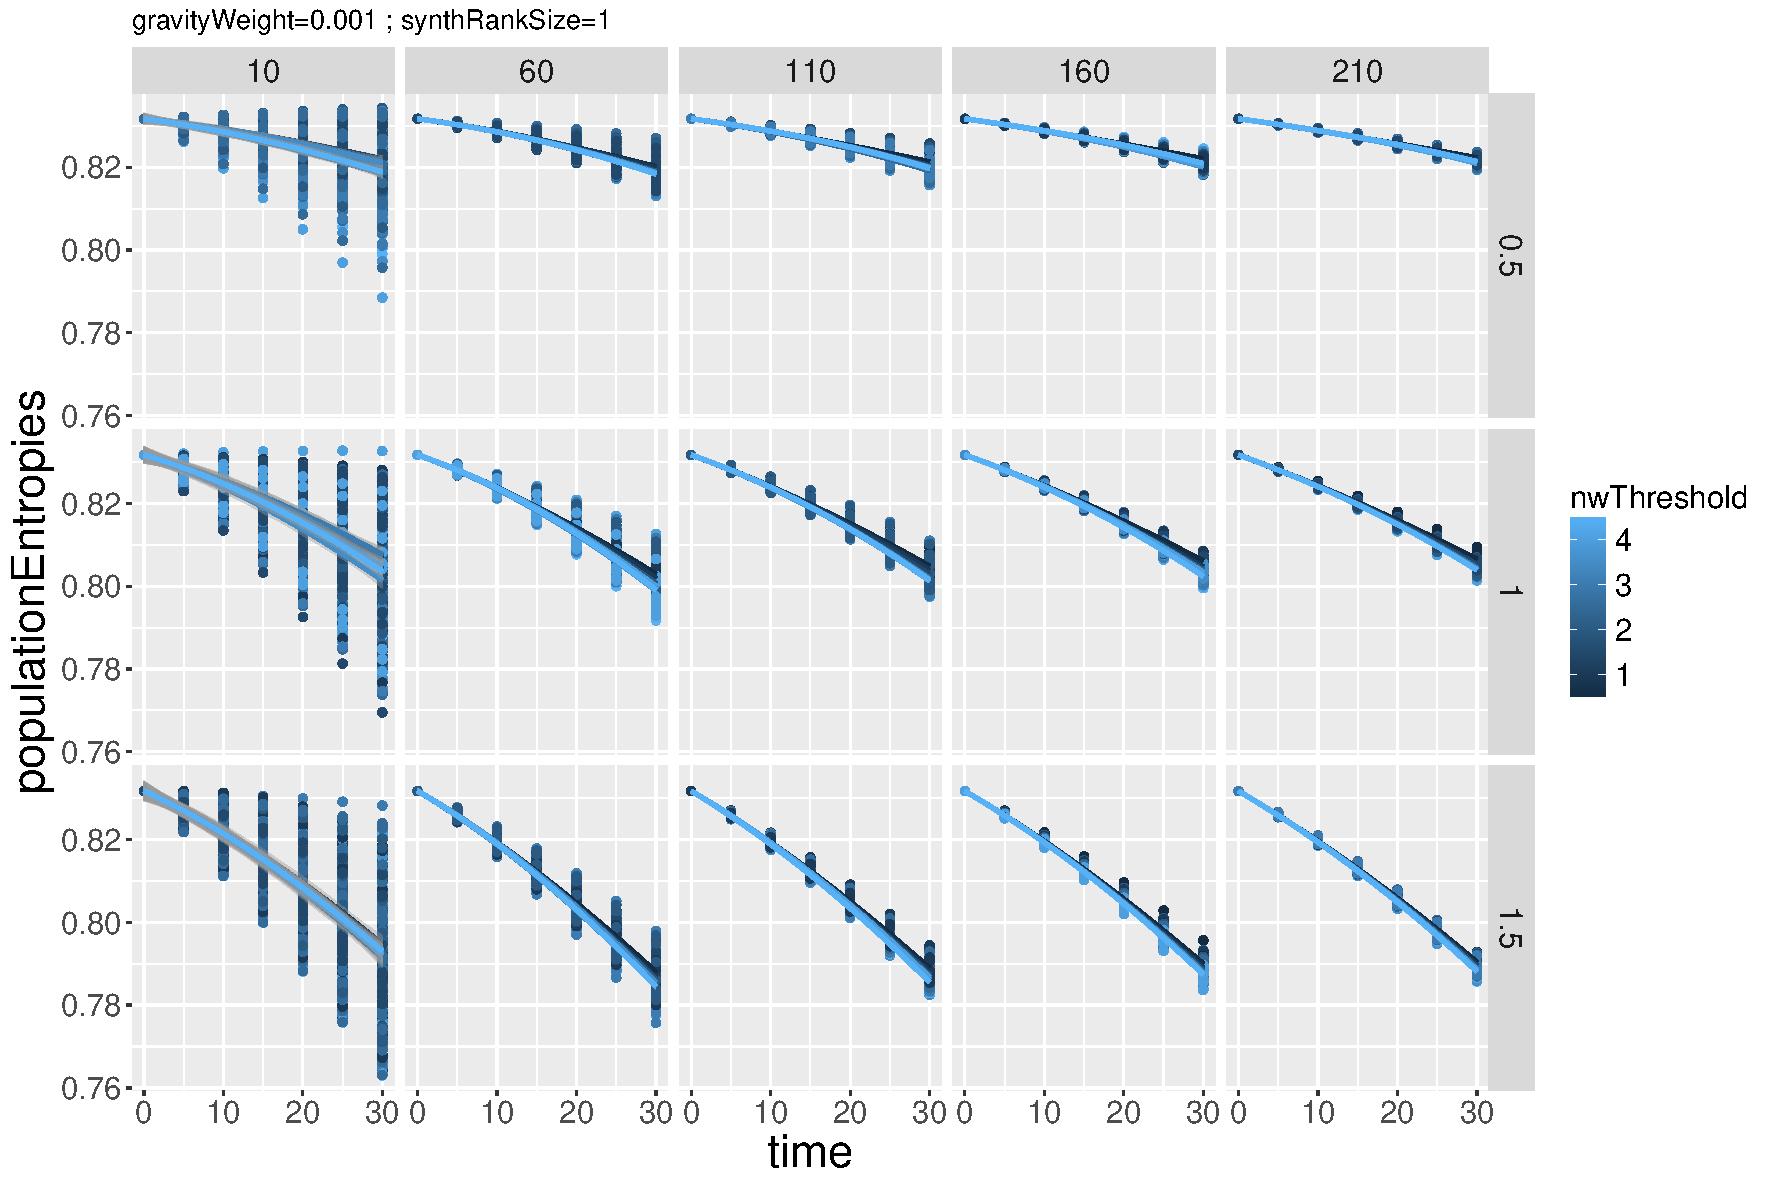
\includegraphics[width=0.48\linewidth]{Figures/MacroCoEvol/populationEntropiessynthRankSize1_gravityWeight0_001.pdf}
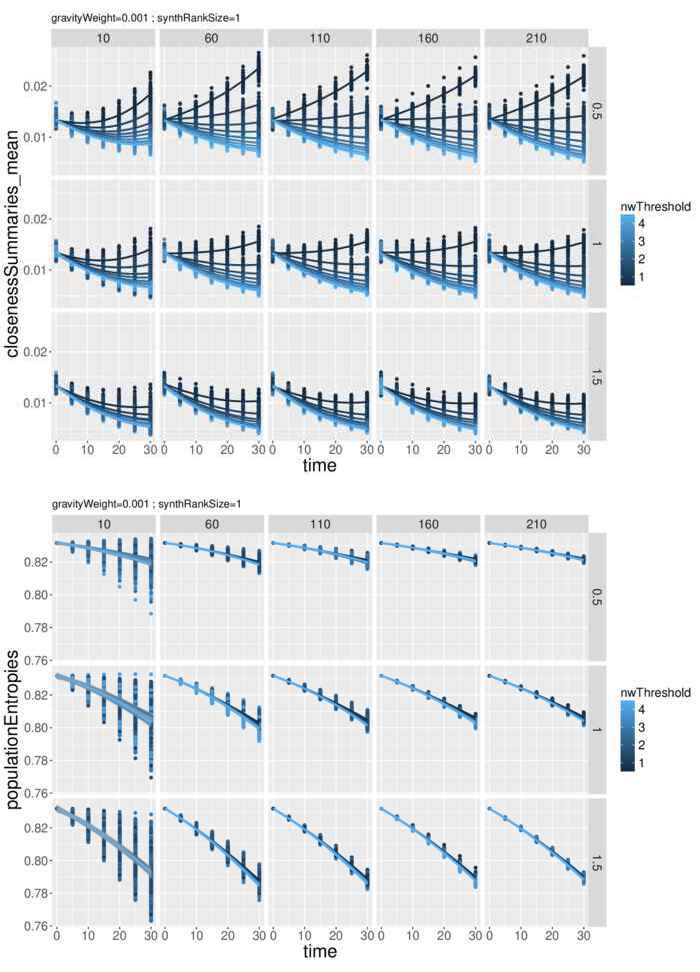
\includegraphics[width=\linewidth,height=0.9\textheight]{Figures/Final/A-macrocoevol-behavior-time.jpg}
\appcaption{\textbf{Behavior of temporal indicators for the co-evolution model at the macroscopic scale.} \textit{(Top)} Average of closeness centralities, as a function of time, for varying $d_G$ (columns), $\gamma_G$ (rows) and $\phi_0$ (color), at fixed $w_G = 0.001$; \textit{(Bottom)} Entropy of populations, as a function of time, for varying $d_G$ (columns), $\gamma_G$ (rows) and $\phi_0$ (color), at fixed $w_G = 0.001$.\label{fig:app:macrocoevol:behavior-time}}{\textbf{Comportement d'indicateurs temporels pour le modèle de co-évolution à l'échelle macroscopique.} \textit{(Haut)} Moyenne des centralités de proximité, en fonction du temps, pour $d_G$ (colonnes), $\gamma_G$ (lignes) et $\phi_0$ (couleur) variables, à $w_G = 0.001$ fixé ; \textit{(Bas)} Entropie des populations, en fonction du temps, pour $d_G$ (colonnes), $\gamma_G$ (lignes) et $\phi_0$(couleur) variables, à $w_G = 0.001$ fixé.\label{fig:app:macrocoevol:behavior-time}}
\end{figure}
%%%%%%%%%%%%%




\bpar{
We give in Fig.~\ref{fig:app:macrocoevol:behavior-aggreg} the behavior of aggregated indicators, namely $C\left[Z_i\right]$ and $\rho_r \left[Z_i\right]$. The complexity of accessibility trajectories mostly varies according to $d_G$, $\gamma_G$ and $\phi_0$ for the low values. The rank correlation of accessibilities is in its turn only sensitive to $d_G$ and $\gamma_G$, what means that differences in network evolution do not perturb the dynamics of the hierarchy of accessibilities.
}{
Nous donnons en Fig.~\ref{fig:app:macrocoevol:behavior-aggreg} le comportement d'indicateurs agrégés, à savoir $C\left[Z_i\right]$ et $\rho_r \left[Z_i\right]$. La complexité des trajectoires d'accessibilité varie principalement selon $d_G$, $\gamma_G$ et $\phi_0$ pour les faibles valeurs. La corrélation de rang des accessibilités est quant à elle uniquement sensible à $d_G$ et $\gamma_G$, ce qui veut dire que des différences d'évolution du réseau ne perturbent pas la dynamique de la hiérarchie des accessibilités.
}



%%%%%%%%%%%%%
\begin{figure}
%\includegraphics[width=0.48\linewidth]{Figures/MacroCoEvol/complexityAccessibility_synthrankSize1_nwGmax0_05}
%\includegraphics[width=0.48\linewidth]{Figures/MacroCoEvol/rankCorrAccessibility_synthrankSize1_nwGmax0_05}
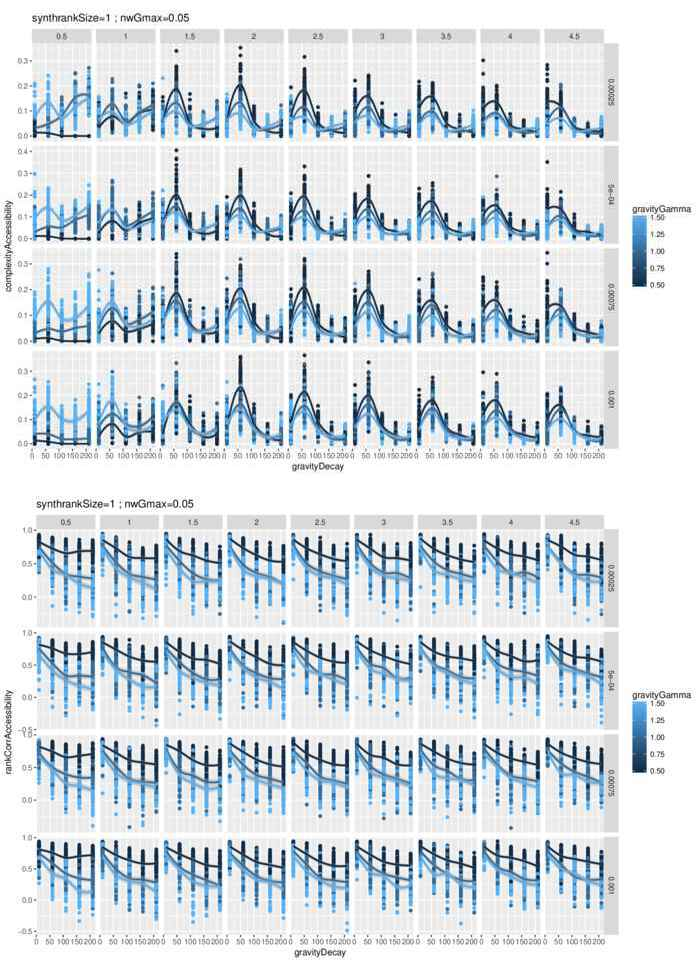
\includegraphics[width=\linewidth,height=0.9\textheight]{Figures/Final/A-macrocoevol-behavior-aggreg.jpg}
\appcaption{\textbf{Behavior of aggregated indicators behavior for the model of coevolution at the macroscopic scale.} \textit{(Top)} Complexxity of accessibilities, as a function of $d_G$, for varying $\phi_0$ (columns), $w_G$ (rows) and $\gamma_G$ (color); \textit{(Bottom)} Rank correlations of accessibilities, for the same parameters.\label{fig:app:macrocoevol:behavior-aggreg}}{\textbf{Comportement d'indicateurs agrégés pour le modèle de co-évolution à l'échelle macroscopique.} \textit{(Haut)} Complexité des accessibilités, en fonction de $d_G$, pour $\phi_0$ (colonnes), $w_G$ (lignes) et $\gamma_G$ (couleur) variables ; \textit{(Bas)} Corrélations de rang des accessibilités, pour les mêmes paramètres.\label{fig:app:macrocoevol:behavior-aggreg}}
\end{figure}
%%%%%%%%%%%%%


\bpar{
The Fig.~\ref{fig:app:macrocoevol:distcorrs} gives the correlations $\rho_d$ as a function of distance deciles for all couples of variables. The strong values of $d_G$ give zero correlations for all values of distance, while $d_G=10$ exhibits local regimes. A constant correlation between centrality and accessibility emerges for an intermediate value $d_G = 60$, what could possibly be put in correspondence with the maximum of complexity for accessibilities which was obtained before.
}{
La Fig.~\ref{fig:app:macrocoevol:distcorrs} donne les corrélations $\rho_d$ en fonction des déciles de distance pour l'ensemble des couples de variables. Les fortes valeurs de $d_G$ donnent des corrélations nulles pour l'ensemble des valeurs de la distance, tandis que $d_G = 10$ témoigne de régimes locaux. Une corrélation constante entre centralité et accessibilité émerge pour une valeur intermédiaire $d_G = 60$, qui est éventuellement à mettre en correspondance avec le maximum de complexité pour les accessibilités obtenu précédemment.
}



%%%%%%%%%%%%%
\begin{figure}
%\includegraphics[width=0.9\linewidth]{Figures/MacroCoEvol/distcorrs_gravityWeight5e-04_nwThreshold4_5}
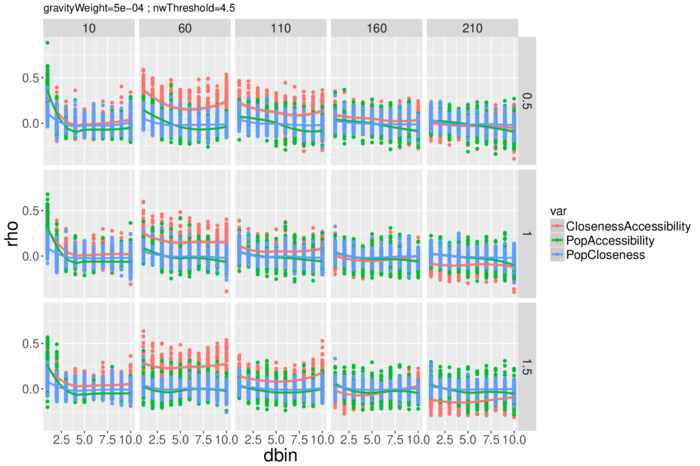
\includegraphics[width=\linewidth]{Figures/Final/A-macrocoevol-distcorrs.jpg}
\appcaption{\textbf{Correlations as a function of distance.} Correlation $\rho_d$ between couples of variables (given by color), as a function of distance $d$ (discretized into deciles), for varying $d_G$ (columns) and varying $\gamma_G$ (rows), at $w_G = 5e-4$ et $\phi_0 = 4.5$.\label{fig:app:macrocoevol:distcorrs}}{\textbf{Corrélations en fonction de la distance.} Correlation $\rho_d$ entre couples de variables (donné par la couleur), en fonction de la distance $d$ (discretisée en déciles), pour $d_G$ variable (colonnes) et $\gamma_G$ variable (lignes), à $w_G = 5e-4$ et $\phi_0 = 4.5$.
\label{fig:app:macrocoevol:distcorrs}}
\end{figure}
%%%%%%%%%%%%%


\bpar{
Finally, the Fig.~\ref{fig:app:macrocoevol:laggedcorrs} gives the lagged correlations $\rho_{\tau}$ for all variable couples. The variations of $\gamma_G$ do not influence much the regimes obtained, on the contrary to $d_G$, for which we observe a continuous variation of the qualitative shape of profiles.
}{
Enfin, la Fig.~\ref{fig:app:macrocoevol:laggedcorrs} donne les corrélations retardées $\rho_{\tau}$ pour l'ensemble des couples de variables. Les variations de $\gamma_G$ influencent peu les régimes obtenus, contrairement à $d_G$, pour lequel on observe une variation continue de la forme qualitative des profils.
}


\bpar{
More precisely, we observe that the correlation between population and accessibility is globally constant, possibly because of the auto-correlation, and does not play a role in the definition of regimes. For large values of $d_G$, we observe a positive deviation of correlations for positive and negative delays for accessibility and centrality. There is in that case circular causality and the model captures a co-evolution in that sense. Accessibility strongly causes centrality for $d_G = 10$, and the trend is inverted for large $d_G$. For $d_G = 10$, we observe a single direction relation of population towards the network. For intermediate regimes, there is directly circularity between population and centrality. Finally, for $d_G . 110$ there is ``indirect circularity'' between population and accessibility, since accessibility causes centrality which causes population.
}{
Plus précisément, nous observons que la corrélation entre population et accessibilité est globalement constante, probablement du fait de l'auto-corrélation, et n'entre pas en jeu dans la définition des régimes. Pour des grandes valeurs de $d_G$, on observe une déviation positive des corrélations pour les délais positifs et négatifs pour accessibilité et centralité. Il y a dans ce cas causalité circulaire et le modèle capture une co-évolution dans ce sens. L'accessibilité cause fortement la centralité pour $d_G = 10$, puis la tendance s'inverse pour les grands $d_G$. Pour $d_G = 10$, nous observons une relation à sens unique de la population vers le réseau. Pour les régimes intermédiaires, il y a circularité directement entre population et centralité. Enfin, pour $d_G > 110$ il y a ``circularité indirecte'' entre population et accessibilité, puisque accessibilité cause centralité qui cause population.
}

\bpar{
This visual exploration is preliminary and is continued by the statistical validation of the different regimes in main text.
}{
Cette exploration visuelle est préliminaire et est continuée par la validation statistique des différents régimes en texte principal.
}



%%%%%%%%%%%%%
\begin{figure}
%\includegraphics[width=0.9\linewidth]{Figures/MacroCoEvol/laggedcorrs_gravityWeight5e-04_nwThreshold4_5}
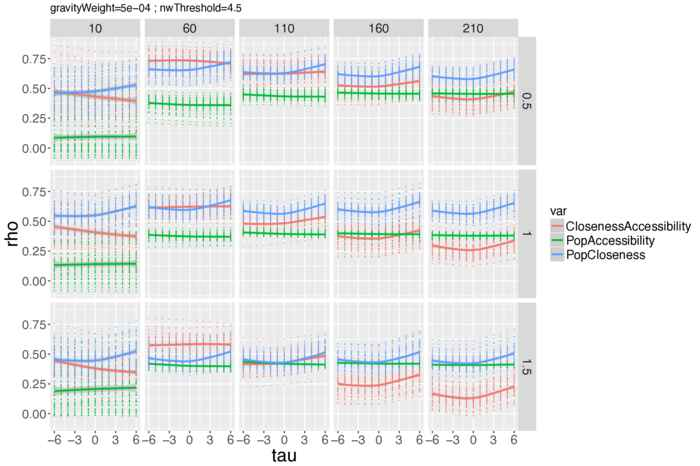
\includegraphics[width=\linewidth]{Figures/Final/A-macrocoevol-laggedcorrs.jpg}
\appcaption{\textbf{Lagged correlations.} Lagged correlations $\rho_{\tau}$ as a function of the delay $\tau$, in a similar way for varying $d_G$ (columns) and $\gamma_G$ (rows), at $w_G = 5e-4$ et $\phi_0 = 4.5$.\label{fig:app:macrocoevol:laggedcorrs}}{\textbf{Corrélations retardées.} Correlations retardées $\rho_{\tau}$ en fonction du retard $\tau$, de manière similaire pour $d_G$ variable (colonnes) et $\gamma_G$ variable (lignes), à $w_G = 5e-4$ et $\phi_0 = 4.5$.
\label{fig:app:macrocoevol:laggedcorrs}}
\end{figure}
%%%%%%%%%%%%%



\subsubsection{Application of the PSE algorithm}{Application de l'algorithme PSE}


\bpar{
The algorithm has been precisely applied with the objectives $\rho_{\tau_{\pm}}\left[x_i,x_j\right] - \rho_0$ with $x_i$ the 3 variables we considered and $i<j$, the estimated correlation being zero if it is non-significant or lower than $\rho_0$ in absolute value. Objectives vary in $\left[-0.2,0.2\right]$ with a step of $0.01$ (in practice, the quasi-totality of obtained values are lower in absolute value to 0.1, since the first and last centiles are lower, except two cases at 0.12 and 0.16).
}{
L'algorithme a été précisément appliqué avec les objectifs $\rho_{\tau_{\pm}}\left[x_i,x_j\right] - \rho_0$ avec $x_i$ les 3 variables considérées et $i<j$, la corrélation estimée étant nulle si non significative ou moins forte que $\rho_0$. Les objectifs varient dans $\left[-0.2,0.2\right]$ avec un pas de $0.01$ (en pratique, la quasi-totalité des valeurs obtenues sont inférieures en valeur absolue à 0.1, puisque les premiers et derniers centiles y sont inférieurs, sauf deux exceptions à 0.12 et 0.16).
}

\bpar{
The algorithm is launched on the grid with 300 parallel islands, each island having a lifetime of 2 hours, for a total of 616 generations.
}{
L'algorithme est lancé sur grille avec 300 îles en parallèle, chaque île ayant une durée de vie de 2 heures, pour un total de 616 générations.
}
% TODO : may have not converged : very low number of generations !


\bpar{
Results of the population obtained are shown as a point cloud in Fig.~\ref{fig:app:macrocoevol:pse}. We observe that the correlation for which the distribution is the most dispersed is $\rho_{\tau_+}\left[\mu_i,c_i\right]$. Furthermore, each couple of correlations has non-reachable quadrants, suggesting impossible behaviors in the model: for example, there is close to no point with a negative causality between population and centrality and a negative causality between centrality and accessibility, these two links being thus not compatible. The couple with which it seems the hardest to extend direct circularities is accessibility and centrality, what suggests a domination of centrality in comparison to population in the expression of accessibility since the link with population has a higher range of freedom.
}{
Les résultats de la population obtenue sont montrés sous forme de nuage de points en Fig.~\ref{fig:app:macrocoevol:pse}. Nous constatons que la corrélation dont la distribution est la plus dispersée est $\rho_{\tau_+}\left[\mu_i,c_i\right]$. Par ailleurs, chaque couple de corrélations possède des cadrants impossibles à atteindre, suggérant des comportements impossibles du modèle : par exemple, il n'y a quasiment aucun point avec une causalité négative entre population et centralité et une causalité négative entre centralité et accessibilité, ces deux liens étant alors incompatibles. Le couple avec lequel il semble le plus dur d'étendre les circularités directes est accessibilité et centralité, ce qui suggère une domination de la centralité par rapport à la population dans l'expression de l'accessibilité puisque le lien avec population possède une plus grande étendue de liberté.
}


\bpar{
Basically, the algorithm unveils a richness of behaviors, extending again the one obtained with the simple exploration.
}{
Principalement, l'algorithme révèle une richesse de comportements étendant encore celle obtenue par l'exploration simple.
}


% quantile(res$rhoPopClosenessPos,c(0.01,0.99))
%%         1%         99% 
%-0.01334991  0.11833861 
% quantile(res$rhoPopClosenessNeg,c(0.01,0.99))
%         1%         99% 
%-0.02443863  0.05279930 
% quantile(res$rhoPopAccessibilityPos,c(0.01,0.99))
%         1%         99% 
%-0.01573526  0.06791604 
% quantile(res$rhoPopAccessibilityNeg,c(0.01,0.99))
%         1%         99% 
%-0.01634579  0.10121212 
% quantile(res$rhoClosenessAccessibilityPos,c(0.01,0.99))
%        1%        99% 
%-0.0141801  0.1586433 
%quantile(res$rhoClosenessAccessibilityNeg,c(0.01,0.99))
%         1%         99% 
%-0.06818126  0.08764040 



%%%%%%%%%%%%%
\begin{figure}
	%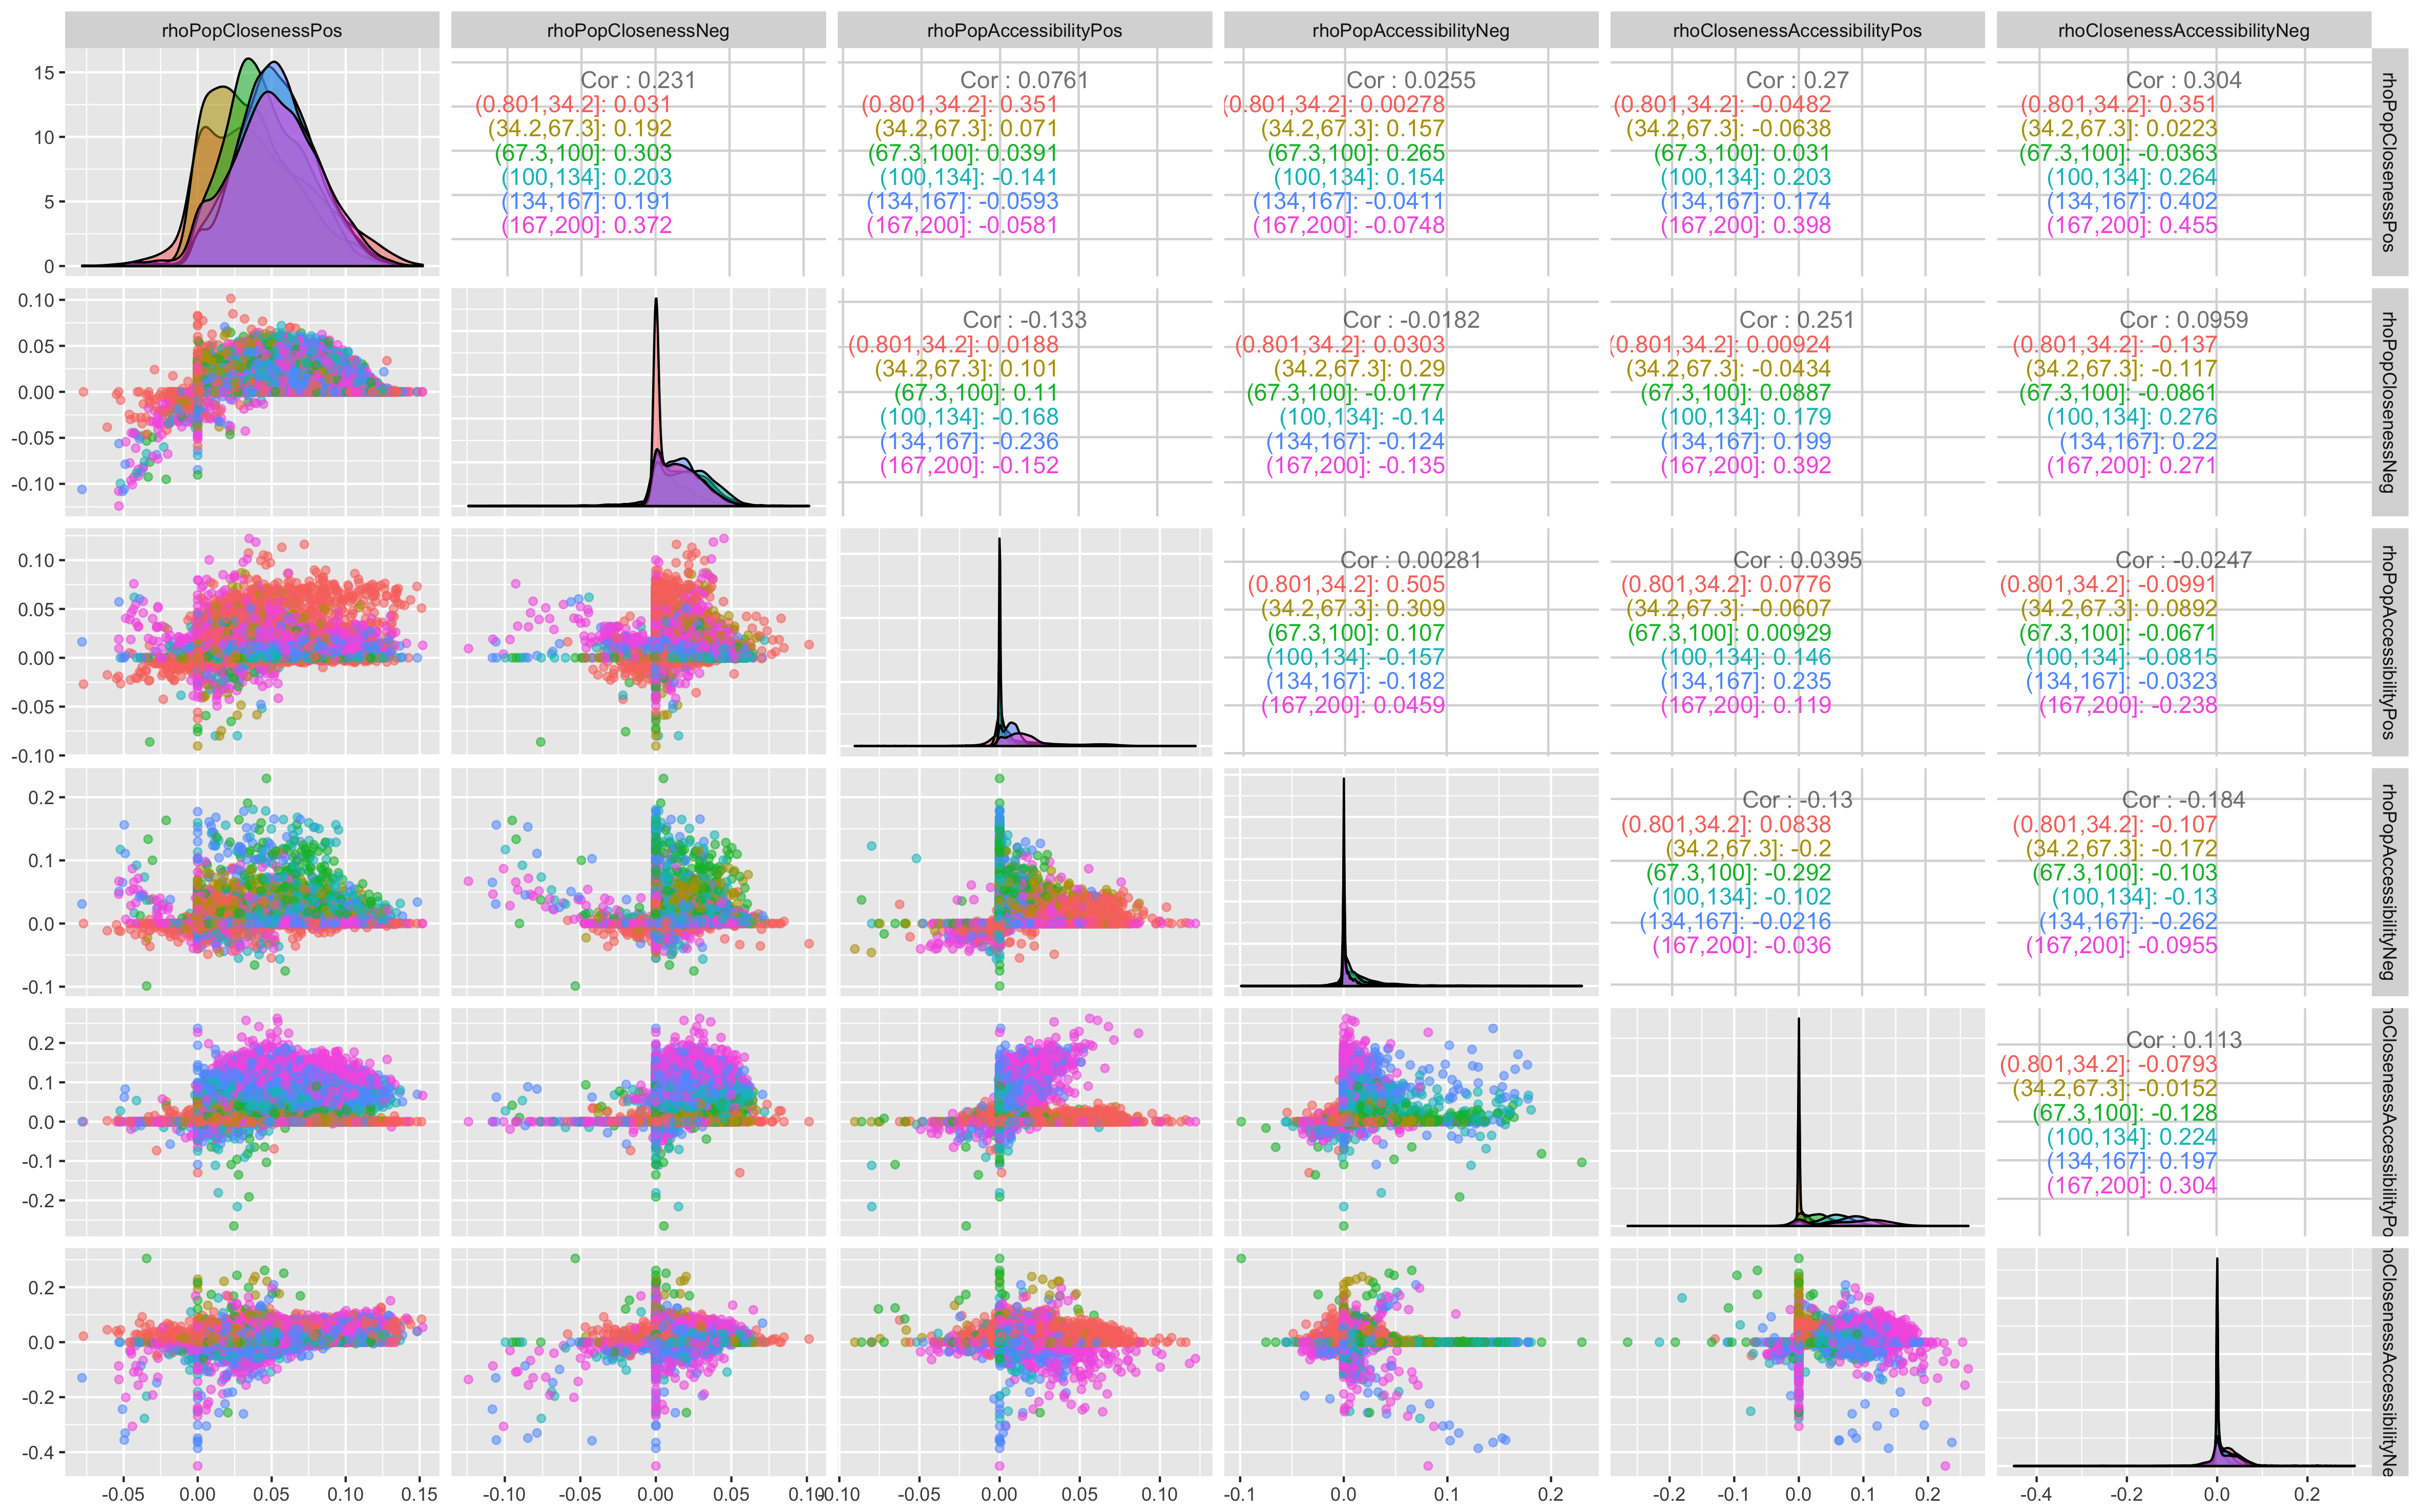
\includegraphics[width=\linewidth]{Figures/MacroCoEvol/scatterplot_colorgravityDecay.png}
	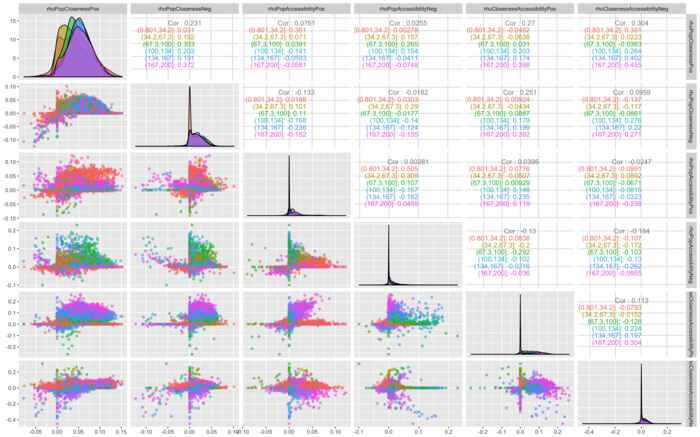
\includegraphics[width=\linewidth]{Figures/Final/A-macrocoevol-pse.jpg}
	\appcaption{\textbf{Application of the PSE algorithm to the macroscopic model}. We give point clouds of optimal lagged correlations, for each couple of variables and the sign of the delay. The color of points gives the value of the $d_G$ parameter, numerical inserts the stratified values of correlations between correlations, and histograms the statistical distribution of each correlation.\label{fig:app:macrocoevol:pse}}{\textbf{Application de l'algorithme PSE au modèle macroscopique}. Nous donnons les nuages de points des corrélations retardées optimales, pour chaque couple de variable et le signe du délai. La couleur des points donne la valeur du paramètre $d_G$, les encarts numériques les valeurs stratifiées des corrélations entre corrélations, et les histogrammes la distribution statistique de chaque corrélation.\label{fig:app:macrocoevol:pse}}
\end{figure}
%%%%%%%%%%%%%






%%%%%%%%%%%%%%%%%%%
\subsection{Real data}{Données réelles}


\bpar{
We give in Fig.~\ref{fig:app:macrocoevol:pareto} the Pareto fronts for the model calibration on real data with the objectives $(\varepsilon_G,\varepsilon_L)$, which are similar to the ones given in~\ref{fig:macrocoevol:pareto}, but here with color giving the value of the $d_G$ parameter. We observe a dichotomy between large values of $d_G$ and low values, for example within the 1946 period, the decrease corresponding to a significant gain for the fit on population. In this case, long-range interactions better correspond to an adjustment of the distance, while population rather follows local processes.
}{
Nous donnons en Fig.~\ref{fig:app:macrocoevol:pareto} les fronts de Pareto pour la calibration du modèle sur données réelles selon $(\varepsilon_G,\varepsilon_L)$, similaires à ceux donnés en~\ref{fig:macrocoevol:pareto}, mais ici avec la couleur donnant la valeur du paramètre $d_G$. Nous constatons une dichotomie entre des grandes valeurs de $d_G$ et des faibles, par exemple au sein de la période 1946, la diminution correspondant à un gain considérable pour la population. Dans ce cas, les interactions lointaines correspondent mieux à un ajustement de la distance, tandis que la population suit plutôt une logique locale.
}


%%%%%%%%%%%%%%%%%%%
\begin{figure}
%\includegraphics[width=0.9\linewidth]{Figures/MacroCoEvol/pareto_gravityDecay}
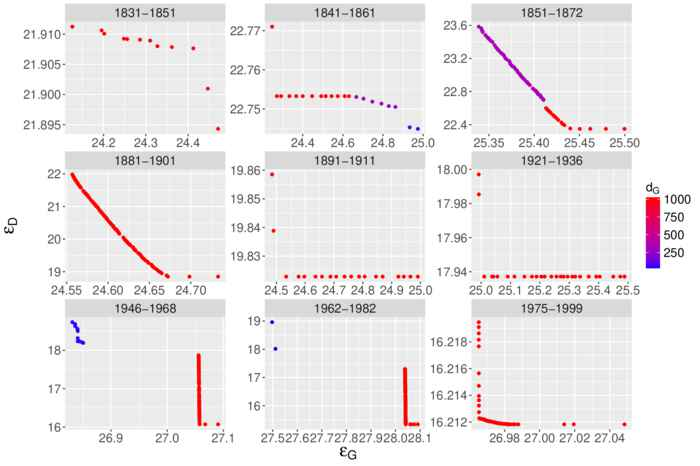
\includegraphics[width=\linewidth]{Figures/Final/A-macrocoevol-pareto.jpg}
\appcaption{\textbf{Pareto fronts for the bi-objective calibration with population and distance.} The fronts are given for each calibration period, and colored as a function of $d_G$.\label{fig:app:macrocoevol:pareto}}{\textbf{Fronts de Pareto pour la calibration bi-objectif population et distance.} Les fronts sont donnés pour chaque période de calibration, et colorés en fonction de $d_G$.\label{fig:app:macrocoevol:pareto}}
\end{figure}
%%%%%%%%%%%%%%%%%%%








